\documentclass[12pt]{article}

\usepackage[dvips,letterpaper,margin=0.75in,bottom=0.5in]{geometry}
\usepackage{cite}
\usepackage{slashed}
\usepackage{graphicx}
\usepackage{amsmath}
\usepackage{braket}
\usepackage[percent]{overpic}

\begin{document}

\section{Introduction}

In this lab, we will build a 4-bit, 400 Hz, microprocessor.  We'll cheat a bit and use the Arduino as the control logic and memory, but we will build the heart of the microprocessor, the arithmetic logic unit, from ICs.  To keep things reasonable, we will build a minimalistic command set that consists of only the NAND operation and a one-bit cyclic shift to the right.

This lab is purely for fun.  Get as far as you can, but there is no need to turn anything in!

\section{Arduino and IC interface}

\begin{figure}[htbp]
\begin{center}
{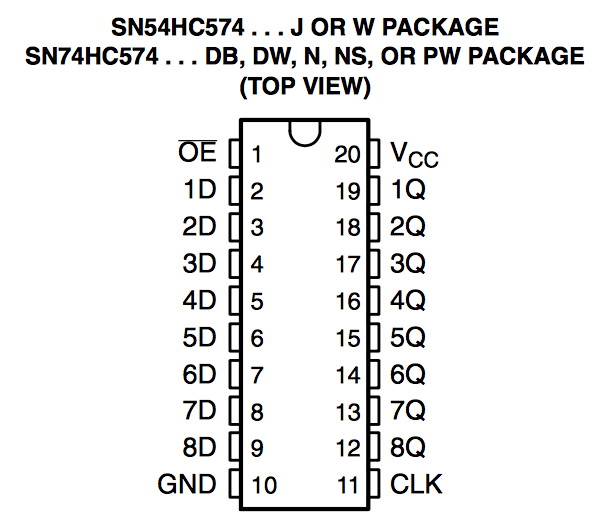
\includegraphics[width=0.40\textwidth]{figs/SN74HC574_pinout.png}}
{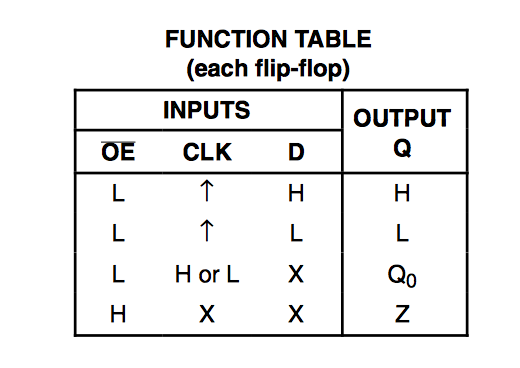
\includegraphics[width=0.25\textwidth]{figs/SN74HC574_table.png}}
{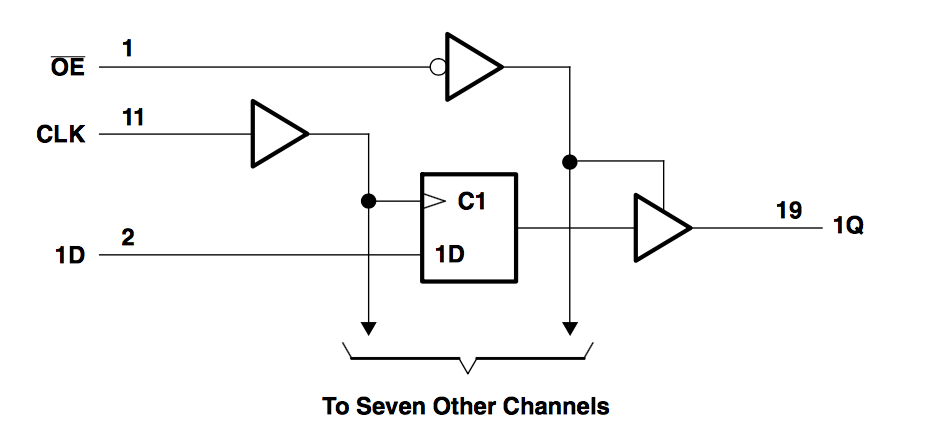
\includegraphics[width=0.50\textwidth]{figs/SN74HC574_diagram.png}}
\end{center}
\caption{\label{fig:hc574} Excerpts from the SN74HC574 datasheet.}
\end{figure}

\begin{figure}[htbp]
\begin{center}
{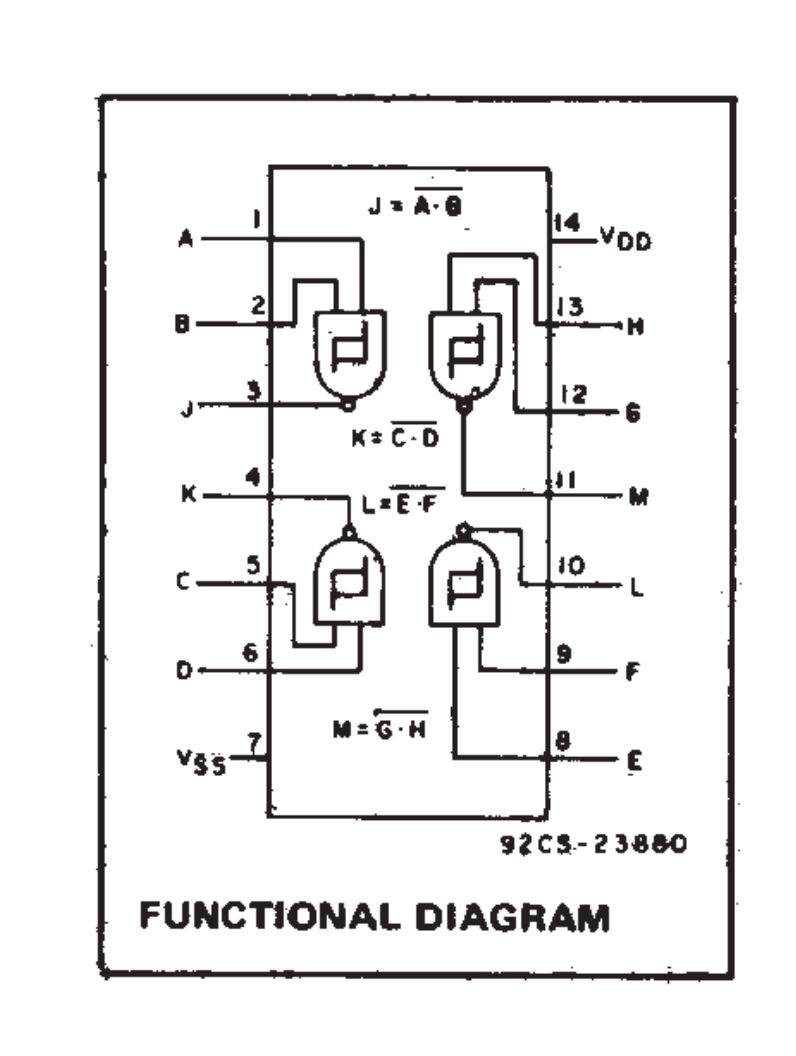
\includegraphics[width=0.40\textwidth]{figs/CD4093B.png}}
\end{center}
\caption{\label{fig:cd4093b} Pinout from the CD4093B datasheet.}
\end{figure}

All of the ICs we will use can be driven by the 5 V output provided by the Arduino.  Use a single breadboard and provide both a ground and 5 V bus for use with your IC components.  The ICs we will use expect ground on the left side, and Vcc on the right side, so you might as well lay it out that way.

We'll rely on two ICs:  an 8-bit D-type edge triggered flip flop (SN74HC574) and a quad NAND 
gate (CD4093B).  The quad NAND does not have an output enable, so we'll drive the data bus from the output of NAND through a resistor (one for each bit).  That way, the NAND output will be available on the bus only if all of the other devices (the Arduino and SHIFT register) are not driving it.  The value of the resistor should be $30~{\rm k \Omega}$, which is large enough not to require too much current from any device driving the data bus, while small enough to produce a negligible voltage drop when the bus is driven (through the resistor) by the NAND device.

The Arduino will read and write the four-bit data bus (DAT0, DAT1, DAT2, and DAT3) as well as provide the control signals needed to drive the ALU.  A common latch signal (LCH) is used to latch data into registers A, B, and C.  An (active low) output enable (OES) is used when the shift register output should be asserted on the data bus.  Though not needed by your ALU, for your convenience when using the scope, the clock signal (CLK) and an appropriate trigger (TRIG) are also provided.  The TRIG signal is generated at the start of each program cycle (when the program counter restarts at zero).  By plugging this signal into the external trigger for your scope, you can look at two other signals simultaneously.
The identification of these logical signals with physical pins on the Arduino is:\\
\begin{center}
\begin{tabular}{ll}
Arduino Pin & Logical Signal \\
2 & CLK \\
4 & TRIG \\
5 & LCH \\
6 & OES \\
8 & DAT0 \\
9 & DAT1 \\
10 & DAT2 \\
11 & DAT3 \\
\end{tabular}
\end{center}
 
The Arduino sketch needed to drive your ALU is provided on the course website:  {\tt alu\_driver.ino}.   It provides three sample programs which you can run on your ALU, which are described in detail below.   Apart from selecting which program to run within the {\tt setup} function, you should not need to modify this sketch, however, you can certainly adjust the test patterns or implement your own programs if you would like.
 
\section{NAND Operation}

%wavedrom.com:
%{signal: [
% {},
% {name: 'CLK', wave: 'n.....'},
%  {name: 'DAT', wave: 'x234x.', data: ['a', 'b', 'out']},
% {name: 'LCH', wave: 'lnnl..'},
%  {name: 'OES', wave: '1.....'},  
%  {},
%  {name: 'CLK', wave: 'n.....'},
 % {name: 'DAT', wave: 'x23x..', data: ['c', 'out']},
 % {name: 'LCH', wave: 'lnl...'},
 % {name: 'OES', wave: '1.01..'}  
%]}

\begin{figure}[htbp]
\begin{center}
%\begin{overpic}[width=0.75\textwidth,grid,tics=5]{timing.png}
\begin{overpic}[width=0.75\textwidth]{figs/timing.png}
\put (35,92) {Nand Operation}
\put (35,42) {Shift Operation}
\end{overpic}
\end{center}
\caption{\label{fig:timing} Control signals for the NAND and SHIFT operations.  For the NAND operation, the registers A and B are clocked in on two successive common latch signals (LCH) and the output is made available on the following clock cycle.  As this bus is driven by the NAND gates through resistors, no output enable signal is needed for the NAND operation, but Arduino must set these pins as input and OES must be high during the entire operation.  For the SHIFT operation, the single register C is clocked in on one common latch signal (LCH) and the SHIFT output is made available on the data bus by the active low output enable shift.}
\end{figure}


\begin{figure}[htbp]
\begin{center}
%\begin{overpic}[width=0.75\textwidth,grid,tics=5]{circuit_nand.pdf}
\begin{overpic}[width=0.75\textwidth]{figs/circuit_nand.pdf}
\put (1,31) {DAT0}
\put (1,42) {LCH}
\put (81,55) {$R$}
\put (35,85) {SN74HC574}
\put (65,85) {CD4093B}
\end{overpic}
\end{center}
\caption{\label{fig:circuit_nand} Single-bit implementation of NAND operation.  Only two inputs of the eight available inputs to the SN74HC574 are shown.  Only one of four NAND gates in the CD4093B is shown.  The remaining inputs and gates are used by DAT1, DAT2, and DAT3.  Use $R=30~{\rm k\Omega}$.  In this diagram, note that intersections only make electrical contact if marked with a dot.}
\end{figure}

For the NAND operation, we will load two four-bit registers, $A$ and $B$ during the first two clock cycles, then output the bitwise NAND of these registers on the third clock cycle.  The timing diagram is shown in Fig.~\ref{fig:timing} and the circuit is shown in Fig.~\ref{fig:circuit_nand}.  To save parts, we'll implement both four-bit registers in a single SN74HC574, which accommodates eight total bits.  To accomplish this, the inputs corresponding to register B are driven directly from the data bus, while the inputs corresponding to register A are driven from the output of register B.  This way, we load the contents of register A first, then, when we load the contents of register B, the contents of A will be copied into register A.  Each bit of $A$ is then sent through a NAND gate along with the corresponding bit from $B$.  The output of each NAND gate is connected back to the corresponding bit for the data bus through a resistor, as described above.  There is no need to turn off the output of register A and B, as the NAND gate is always on, so we simply connect the active low output enable ($\bar{OE}$) to ground.

I recommend implementing only a single bit (corresponding to DAT0) of the NAND operation first.  You can debug it using the {\tt nand\_demo} program available in the ALU driver Arduino sketch.  The timing of the common latch signal (LCH) is shown on Fig.~\ref{fig:lch}.  The register A and B are loaded during each pair of rising edges to the latch signal.  The NAND output is then read on the following (third) clock cycle.  This is repeated for four distinct test patterns:\\
\begin{center}
\begin{tabular}{llllll}
A & B & O & A0 & B0 & O0 \\
0b1100 & 0b1010 & 0x7 & 0 & 0 & 1 \\
0b0110 & 0b0101 & 0xB & 0 & 1 & 1 \\
0b0011 & 0b1010 & 0xD & 1 & 0 & 1 \\
0b1001 & 0b0101 & 0xE & 1 & 1 & 0 \\
\end{tabular}
\end{center}
When viewing the DAT0 signal on the scope, you should therefore see two input bits and one output bit for each pattern, i.e. 001,011,101,110 as shown in Fig.~\ref{fig:nandout}, which you interpret as 0 NAND 0 is 1, 0 NAND 1 is 1, 1 NAND 0 is 1, 1 NAND 1 is 0.  

When you have all four bits implemented, you should be able to see the correct four bit NAND output (0x7, 0xB, 0xD, OxE) saved at memory address 64,65,66, and 67, as reported in the Serial Monitor for the Arduino.

\begin{figure}[htbp]
\begin{center}
\begin{overpic}[width=0.75\textwidth,grid,tics=10]{figs/latch.jpg}
\put (37,63) {CLK}
\put (37,25) {LCH}
\end{overpic}
\end{center}
\caption{\label{fig:lch} Latch signal relative to clock during NAND demo program.}
\end{figure}

\begin{figure}[htbp]
\begin{center}
\begin{overpic}[width=0.75\textwidth,grid,tics=10]{figs/nand.jpg}
\put (37,63) {DAT0}
\put (37,34) {DAT1}
\put (6,50) {0}
\put (12,50) {0}
\put (18,50) {1}
\put (26,50) {1}
\put (32,50) {0}
\put (38,50) {1}
\put (45,50) {0}
\put (51,50) {1}
\put (57,50) {1}
\put (65,50) {1}
\put (71,50) {1}
\put (77,50) {0}
\put (6,21) {0}
\put (12,21) {1}
\put (18,21) {1}
\put (26,21) {1}
\put (32,21) {0}
\put (38,21) {1}
\put (45,21) {1}
\put (51,21) {1}
\put (57,21) {0}
\put (65,21) {0}
\put (71,21) {0}
\put (77,21) {1}

\end{overpic}
\end{center}
\caption{\label{fig:nandout} DAT0 and DAT1 output for one full cycle of the NAND demo.}
\end{figure}


\section{SHIFT Operation}

We also provide a cyclic shift operation (e.g. $0001 \to 0010$, $1101 \to 1011$).  This operation requires only one four-bit operand, so only two clock cycles are needed.  On the first clock cycle the four-bit register C is latched by the common latch signal (LCH).  On the second clock cycle, the active low output enable signal for shift (OES) turns on the output of the register C, which drives the data bus, but with each bit shifted by one.  The circuit is shown in Fig.~\ref{fig:circuit_shift}.  We use a second SN74HC574 device, or which we use only four of the eight bits.  

The shift operation can be exercised by using the {\tt shift\_demo} program, which applies the shift operation to the following test patterns:
\begin{center}
\begin{tabular}{llllll}
C & O & C0 & O0 & C1 & O1 \\
0b0001 & 0b0010 (2) & 1 & 0 & 0 & 1 \\
0b0010 & 0b0100 (4) & 0 & 0 & 1 & 0 \\
0b0100 & 0b1000 (8) & 0 & 0 & 0 & 0 \\
0b1000 & 0b0001 (1) & 0 & 1 & 0 & 0 \\
\end{tabular}
\end{center}
When debugging with the scope you should see the corresponding sequence of inputs and outputs as shown in Fig.~\ref{fig:shiftout}.
On the serial port output, you should see the correct shift operation output (2,4,8,1) at addresses 67,68,69,70.

\begin{figure}[htbp]
\begin{center}
%\begin{overpic}[width=0.55\textwidth,grid,tics=5]{circuit_shift.pdf}
\begin{overpic}[width=0.55\textwidth]{figs/circuit_shift.pdf}
\put (2,33) {DAT0}
\put (2,50.33) {DAT1}
\put (2,67.66) {DAT2}
\put (2,85) {DAT3}
\put (2,29.66) {LCH}
\put (2,26) {OES}
\put (28,93) {SN74HC574}
\end{overpic}
\end{center}
\caption{\label{fig:circuit_shift} Complete (four-bit) implementation of the SHIFT operation.  Four inputs of the SN74HC574 are left unused.}
\end{figure}

\begin{figure}[htbp]
\begin{center}
\begin{overpic}[width=0.75\textwidth,grid,tics=10]{figs/shift.jpg}
\put (37,63) {DAT0}
\put (37,32) {DAT1}
\put (6,50) {1}
\put (12,50) {0}
\put (18,50) {0}
\put (26,50) {0}
\put (32,50) {0}
\put (38,50) {0}
\put (45,50) {0}
\put (51,50) {1}
\put (6,25) {0}
\put (12,25) {1}
\put (18,25) {1}
\put (26,25) {0}
\put (32,25) {0}
\put (38,25) {0}
\put (45,25) {0}
\put (51,25) {0}
\end{overpic}
\end{center}
\caption{\label{fig:shiftout} DAT0 and DAT1 output for one full cycle of the SHIFT demo.}
\end{figure}

\section{Add Operation}

Once you have the SHIFT and NAND operation implemented, your ALU is "fully functional".  Well, in fact, we could even have gotten by without the shift operation, but life would be really really painful.  With the shift operation, life is only really painful.  But fortunately for you, the painful addition algorithm, using only SHIFT and NAND, has already been implemented by the {\tt add} program.  Try it out.  If you see the correct sum at the output address 152, you are now making a user specified generic computation on a digital device which you built, which is really no small feat.  Much of our modern world relies on these devices!

\end{document}


